%% Version 4.3.1, 19 May 2014
%
%%%%%%%%%%%%%%%%%%%%%%%%%%%%%%%%%%%%%%%%%%%%%%%%%%%%%%%%%%%%%%%%%%%%%%
% Template.tex --  LaTeX-based template for submissions to the 
% American Meteorological Society
%
% Template developed by Amy Hendrickson, 2013, TeXnology Inc., 
% amyh@texnology.com, http://www.texnology.com
% following earlier work by Brian Papa, American Meteorological Society
%
% Email questions to latex@ametsoc.org.
%
%%%%%%%%%%%%%%%%%%%%%%%%%%%%%%%%%%%%%%%%%%%%%%%%%%%%%%%%%%%%%%%%%%%%%
% PREAMBLE
%%%%%%%%%%%%%%%%%%%%%%%%%%%%%%%%%%%%%%%%%%%%%%%%%%%%%%%%%%%%%%%%%%%%%

%% Start with one of the following:
% DOUBLE-SPACED VERSION FOR SUBMISSION TO THE AMS
%\documentclass{ametsoc}

% TWO-COLUMN JOURNAL PAGE LAYOUT---FOR AUTHOR USE ONLY
\documentclass[twocol]{ametsoc}

%%%%%%%%%%%%%%%%%%%%%%%%%%%%%%%%
%%% To be entered only if twocol option is used

\journal{jcli}

%  Please choose a journal abbreviation to use above from the following list:
% 
%   jamc     (Journal of Applied Meteorology and Climatology)
%   jtech     (Journal of Atmospheric and Oceanic Technology)
%   jhm      (Journal of Hydrometeorology)
%   jpo     (Journal of Physical Oceanography)
%   jcli      (Journal of Climate)
%   mwr      (Monthly Weather Review)
%   wcas      (Weather, Climate, and Society)
%   waf       (Weather and Forecasting)
%   bams (Bulletin of the American Meteorological Society)
%   ei    (Earth Interactions)

%%%%%%%%%%%%%%%%%%%%%%%%%%%%%%%%
%Citations should be of the form ``author year''  not ``author, year''
\bibpunct{(}{)}{;}{a}{}{,}

%%%%%%%%%%%%%%%%%%%%%%%%%%%%%%%%

%%% To be entered by author:

%% May use \\ to break lines in title:

\title{Atmospheric response to simulated historical sea ice loss}

%%% Enter authors' names, as you see in this example:
%%% Use \correspondingauthor{} and \thanks{Current Affiliation:...}
%%% immediately following the appropriate author.
%%%
%%% Note that the \correspondingauthor{} command is NECESSARY.
%%% The \thanks{} commands are OPTIONAL.

    %\authors{Author One\correspondingauthor{Author One, 
    % American Meteorological Society, 
    % 45 Beacon St., Boston, MA 02108.}
% and Author Two\thanks{Current affiliation: American Meteorological Society, 
    % 45 Beacon St., Boston, MA 02108.}}

\authors{Kelly E. McCusker\correspondingauthor{School of Earth and Ocean Sciences, University of Victoria, Victoria, BC, Canada.}}

%% Follow this form:
    % \affiliation{American Meteorological Society, 
    % Boston, Massachusetts.}

\affiliation{University of Victoria,
                      Victoria, British Columbia}

%% Follow this form:
    %\email{latex@ametsoc.org}

\email{kemccusk@uvic.ca}

%% If appropriate, add additional authors, different affiliations:
    %\extraauthor{Extra Author}
    %\extraaffil{Affiliation, City, State/Province, Country}

\extraauthor{John C. Fyfe}
%\extraaffil{}

%% May repeat for a additional authors/affiliations:

\extraauthor{Michael Sigmond}
\extraaffil{University of Victoria,
                      Victoria, British Columbia}



%%%%%%%%%%%%%%%%%%%%%%%%%%%%%%%%%%%%%%%%%%%%%%%%%%%%%%%%%%%%%%%%%%%%%
% ABSTRACT
%
% Enter your Abstract here

\abstract{Changes in Arctic sea ice play an important role in modulating surface fluxes of heat and moisture, and therefore local near-surface temperatures and precipitation. Whether or not historical sea-ice retreat has had a marked influence on weather patterns, particularly outside the local region, remains an open and important question. Here the effect historical sea-ice loss has on the atmosphere is isolated by prescribing observed sea-ice concentrations and local sea surface temperatures in an atmosphere model. A suite of 120-year simulations is carried out to temper natural variability. We find that observed boundary conditions produce a lowering of Arctic sea level pressure in Autumn that is robust and consistent with other studies, but no clear signal in patterns of variability emerge. Furthermore, the response to observed sea-ice changes is compared to a suite of simulations in which boundary conditions are obtained from an ensemble of historical simulations from a coupled global climate model. We find that whereas near-surface temperature responds in accordance with the amount of sea ice loss --- more loss yields larger warming --- sea-level pressure and geopotential heights remain slave to natural variability. Individual ensemble members have regions and seasons of statistically significant circulation changes in response to sea-ice loss, however those regions and seasons are not robust across ensemble members. Thus, it is likely that 1. historical sea-ice loss played a minimal role in setting circulation trends and 2. any detectable effect sea-ice loss had is due to @@ Thus, caution must be taken when interpreting even long time-slice simulations  @@. Notably, the observed forcing produces a response that is outside the bounds of the } % Harder to tease out is how changes in sea ice influence local and remote circulation. % natural variability for determining both the sea-ice forcing pattern and the response to sea-ice loss by prescribing an ensemble of boundary conditions obtained from a coupled model's ensemble of historical simulations. %...@@. The importance of the pattern of sea-ice loss is further examined by prescribing a suite of boundary conditions obtained from a coupled model's ensemble of historical simulations. 

\begin{document}

%% Necessary!
\maketitle


%%%%%%%%%%%%%%%%%%%%%%%%%%%%%%%%%%%%%%%%%%%%%%%%%%%%%%%%%%%%%%%%%%%%%
% MAIN BODY OF PAPER
%%%%%%%%%%%%%%%%%%%%%%%%%%%%%%%%%%%%%%%%%%%%%%%%%%%%%%%%%%%%%%%%%%%%%
%

%% In all cases, if there is only one entry of this type within
%% the higher level heading, use the star form: 
%%
% \section{Section title}
% \subsection*{subsection}
% text...
% \section{Section title}

%vs

% \section{Section title}
% \subsection{subsection one}
% text...
% \subsection{subsection two}
% \section{Section title}

%%%
% \section{First primary heading}

% \subsection{First secondary heading}

% \subsubsection{First tertiary heading}

% \paragraph{First quaternary heading}

\section{Introduction}

Arctic sea ice has made a dramatic transformation over the late 20th and early 21st century due in large part to increasing greenhouse gas concentrations. Sea ice concentrations are at record lows since at least 1900@@, multi-year ice is declining, and the ice overall is thinner. These changes are both caused by greenhouse warming and help to amplify greenhouse warming in the high northern latitudes such that the Arctic is warming at a rate 2-3 times as large as the rest of the globe (@@). The reduction in sea-ice area unmasks the ocean below, allowing more heat to flux from the warmer waters to the relatively cold atmosphere. The question remains as to how large of an influence this loss of sea ice has on the atmosphere, both locally and remotely.

Much study has 

An important question

Lit review here.
Studies that implement time-slice simulations with similar prescribed boundary conditions from comparable time periods 

It is worth noting that the vast majority of previous studies investigating the response of the atmosphere to changes in sea ice have been accomplished under two model lineages: National Center for Atmospheric Research Community atmosphere models, and atmosphere models developed by the Hadley Centre. Thus, a primary motivation for undertaking this study is to add a much-needed third data point from the Canadian Centre for Climate Modelling and Analysis atmosphere model to the growing literature about the influence of sea ice loss on the atmosphere. Moreover, 

\section{Model and simulations}

To isolate the effect of sea ice on the atmosphere, we use the Canadian Centre for Climate Modelling and Analysis fourth-generation atmosphere general circulation model (CanAM4) with prescribed surface boundary conditions and a freely evolving atmosphere. The model is run at T63 horizontal resolution with 37 vertical levels from the surface up to 1hPa. Further model details can be found in @@cite. We execute a suite of 121-year time-slice simulations and analyze the last 120 years in the results. Each simulation is prescribed with an annually repeating seasonal cycle of sea-ice concentration (SIC), sea-ice thickness (SIT), and sea surface temperatures (SST) as described below. The greenhouse gas, tropospheric aerosol, and solar levels are set to 1984 conditions for all simulations. In this way, any resulting changes in climate can be attributed to changes in the prescribed surface forcing alone.

% boundary conditions
\subsection{Boundary conditions}
\subsubsection{Historical observations}

In order to investigate the effect of observed sea ice loss on the atmosphere, we utilize gridded sea-ice concentration and sea surface temperature data prepared by the Hadley Centre (Hadley Centre sea ice and SST dataset, version 1.1; HadISST1.1). While HadISST1.1 has some known biases @@cite, it is somewhat of an "industry standard" and has been used as boundary conditions for IPCC Atmosphere Model Intercomparison Projects (AMIP) as well as previous work attempting to tease out the effect of sea ice loss on the atmosphere @@cite. The effect of sea ice loss is examined over the satellite era, from 1979 onwards, when the observations are most reliable and the changes in sea ice are greatest. As such, to force the atmosphere model, we calculate monthly mean climatologies of HadISST1.1 sea-ice concentration and SST for the mean of years 1979-1989 as the baseline, and 2002-2011 as the perturbation period. These monthly climatologies are used as repeating boundary conditions in CanAM4 for 121 years, as described next. Because the boundary conditions are annually repeating and the atmosphere has a short memory on the timescale of days (@@), each year can be considered an independent realization of the state of the atmosphere. Thus, after throwing out the first year for spin-up, the ensemble size, N, of each simulation is 120. 

The control simulation with observed boundary conditions is forced with a repeating HadISST1.1 1979-1989 monthly climatology of SIC and SST and is known as \textbf{CTLobs}. CTLobs sea ice thickness boundary condition data is obtained from the output of a previous CanAM model version (@@). The perturbation simulation, known as \textbf{PTobs}, is forced with a repeating HadISST1.1 2002-2011 monthly climatology of SIC, and 1979-1989 SST everywhere except where SIC declines by 10\% or more, in which case SST is the 2002-2011 climatology. In this way, only changes in SST directly attributed to changes in sea ice are incorporated. This method has been previously used in Screen@@, Peings and Magnusdottir@@. The PTobs SIT boundary condition is the same as for CTLobs, except that where SIC disappears, SIT is set to zero @@. We discuss the relative importance of including changes in both local SST and sea-ice thickness in Section @@.

Unless otherwise noted, results will be presented as anomalies from the 120-year average of CTLobs. When looked at in this way, the forcing is effectively the anomaly patterns of sea-ice concentration, thickness, and SST. 
 
\subsubsection{Historical model simulations}

 We contrast results obtained from forcing with observed sea ice and SST conditions with those 

 obtained from  and historical simulations of the second generation Canadian Earth System Model (CanESM2).
% HadISST1.1 ref: http://www.esrl.noaa.gov/psd/data/gridded/data.hadsst.html (not sure it was obtained here...)
% Rayner, N. A.; Parker, D. E.; Horton, E. B.; Folland, C. K.; Alexander, L. V.; Rowell, D. P.; Kent, E. C.; Kaplan, A. (2003) Global analyses of sea surface temperature, sea ice, and night marine air temperature since the late nineteenth century J. Geophys. Res.Vol. 108, No. D14, 4407 10.1029/2002JD002670 

\begin{table*}[t]
\caption{Model simulations. Sensitivity simulations are listed at the bottom of the table.}\label{simstbl}
\begin{center}
\begin{tabular}{lccccccc}
\hline\hline
Exp & SIC & SIT & SST & BC Source & Notes\\
\hline
 CTLobs & 1979-89 & 1979-89 & 1979-89 & HadISST1.1 \\
 PTobs & 2002-11 & 1979-89* & 2002-11 & HadISST1.1 & *SIT set to 0 where SIC 0 and @@\\
 CTLavg & 1979-89 & 1979-89 & 1979-89 & CanESM2 historical ensemble average\\
 PTavg & 2002-12 & 2002-12 & 2002-12 &  CanESM2 historical ensemble average\\
 CTLe1-5 & 1979-89 & 1979-89 & 1979-89  & CanESM2 historical ensemble members 1-5\\
 PTe1-5 & 2002-12 & 2002-12 & 2002-12 &  CanESM2 historical ensemble members 1-5\\
 \hline
 PTavgnosit & 2002-12 & 1979-89* & 2002-12 &  CanESM2 historical ensemble average & *SIT set to 0 where SIC 0. \\
 PTavgnosst & 2002-12 & 2002-12 & 1979-89 &  CanESM2 historical ensemble average & \\
\hline
\end{tabular}
\end{center}
\end{table*}

Add Figure of BCs! SIC, SIT, SST seasonal maps?? @@

\section{Results}

\begin{enumerate}
\item Observational BCs
	\begin{itemize}
	\item a. Describe HadISST results compared to previous studies.
    	\item b. NSIDC results compared to previous studies.
	\item c. HadISST compared to NSIDC. importance of correct trend (?). importance of pattern (?). transition to diff pattern from CanESM

	\item Figures:
		\begin{itemize}
		\item F1. Sea cycle of surface flux, SIC, SST (have mod runs too?)
	 	\item F2. Fall + Winter NH SAT, SLP, Z500? for Had and NSIDC	
		\item F3. Vertical Fall + Winter T, Z, U for Had and NSIDC	
		\end{itemize}
	\end{itemize}

\item Model BCs
	\begin{itemize}
	\item a. Compare HadISST/NSIDC to averageBC simulation, PERT3??
	\item b. Model BCs with and without SST change, SIT change (sensitivity runs, short section?)
	
	\item Figures:
		\begin{itemize}
		\item F4. Fall + Winter NH SAT, SLP, Z500? for PERT1, PERT2, PERT3? (4x3)
		\item F5. Vertical Fall + Winter T, Z, U for sensitivity runs (OR zonalmean with all sims including E runs?)  
                       \end{itemize}
	
	
	\item c. Put averageBC, Had/NSIDC in context using E1-5 and mean of E's
		\begin{itemize}
		\item How robust is each pattern of response? (pattern corr) How much does pattern of forcing matter?
		\item spread of E members is still smaller than uncertainty in time
		\item HadISST out of bounds of our model --> responses are different, so models may not be capturing proper historical circ response (?)
		\item Robust signal in N Atlantic DJF across almost all members --> what is this and what does it mean? 
		\end{itemize}

	\item d. Near-future confirms DJF Z signal

	\end{itemize}

\end{enumerate}


\begin{figure*}[t]
  \noindent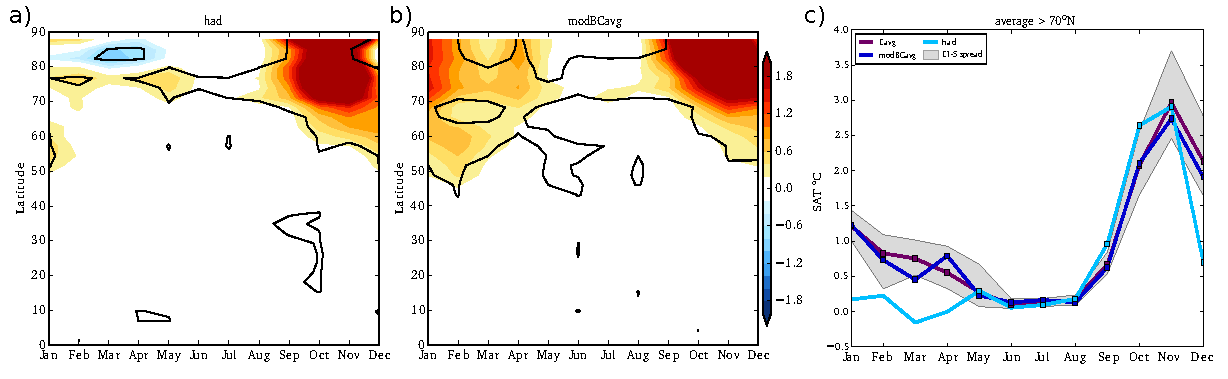
\includegraphics[width=39pc,angle=0]{SAT.pdf}\\
  \caption{Zonal mean surface air temperature anomalies ($^\circ$C) for a.) PTobs-CTLobs, b.) PTavg-CTLavg. c.) Seasonal cycle of area-averaged SAT North of 70$^\circ$N for all PT simulations and their respective CTL simulations. The gray shading indicates the range of e1-5 ensemble members. Note that here 'obs' indicates the simulations run with boundary conditions derived from observations (HadISST1.1).
}\label{f1}
\end{figure*}

%%%%%%%%%%%%%%%%%%%%%%%%%%%%%%%%%%%%%%%%%%%%%%%%%%%%%%%%%%%%%%%%%%%%%
% ACKNOWLEDGMENTS
%%%%%%%%%%%%%%%%%%%%%%%%%%%%%%%%%%%%%%%%%%%%%%%%%%%%%%%%%%%%%%%%%%%%%
%
\acknowledgments
Start acknowledgments here.

%%%%%%%%%%%%%%%%%%%%%%%%%%%%%%%%%%%%%%%%%%%%%%%%%%%%%%%%%%%%%%%%%%%%%
% APPENDIXES
%%%%%%%%%%%%%%%%%%%%%%%%%%%%%%%%%%%%%%%%%%%%%%%%%%%%%%%%%%%%%%%%%%%%%
%
% Use \appendix if there is only one appendix.
%\appendix

% Use \appendix[A], \appendix}[B], if you have multiple appendixes.
%\appendix[A]

%% Appendix title is necessary! For appendix title:
%\appendixtitle{}

%%% Appendix section numbering (note, skip \section and begin with \subsection)
% \subsection{First primary heading}

% \subsubsection{First secondary heading}

% \paragraph{First tertiary heading}

%% Important!
%\appendcaption{<appendix letter and number>}{<caption>} 
%must be used for figures and tables in appendixes, e.g.,
%
%\begin{figure}
%\noindent\includegraphics[width=19pc,angle=0]{figure01.pdf}\\
%\appendcaption{A1}{Caption here.}
%\end{figure}

%%%%%%%%%%%%%%%%%%%%%%%%%%%%%%%%%%%%%%%%%%%%%%%%%%%%%%%%%%%%%%%%%%%%%
% REFERENCES
%%%%%%%%%%%%%%%%%%%%%%%%%%%%%%%%%%%%%%%%%%%%%%%%%%%%%%%%%%%%%%%%%%%%%
% Make your BibTeX bibliography by using these commands:
% \bibliographystyle{ametsoc2014}
% \bibliography{references}


%%%%%%%%%%%%%%%%%%%%%%%%%%%%%%%%%%%%%%%%%%%%%%%%%%%%%%%%%%%%%%%%%%%%%
% TABLES
%%%%%%%%%%%%%%%%%%%%%%%%%%%%%%%%%%%%%%%%%%%%%%%%%%%%%%%%%%%%%%%%%%%%%
%% Enter tables at the end of the document, before figures.
%%
%
%\begin{table}[t]
%\caption{This is a sample table caption and table layout.  Enter as many tables as
%  necessary at the end of your manuscript. Table from Lorenz (1963).}\label{t1}
%\begin{center}
%\begin{tabular}{ccccrrcrc}
%\hline\hline
%$N$ & $X$ & $Y$ & $Z$\\
%\hline
% 0000 & 0000 & 0010 & 0000 \\
% 0005 & 0004 & 0012 & 0000 \\
% 0010 & 0009 & 0020 & 0000 \\
% 0015 & 0016 & 0036 & 0002 \\
% 0020 & 0030 & 0066 & 0007 \\
% 0025 & 0054 & 0115 & 0024 \\
%\hline
%\end{tabular}
%\end{center}
%\end{table}

%%%%%%%%%%%%%%%%%%%%%%%%%%%%%%%%%%%%%%%%%%%%%%%%%%%%%%%%%%%%%%%%%%%%%
% FIGURES
%%%%%%%%%%%%%%%%%%%%%%%%%%%%%%%%%%%%%%%%%%%%%%%%%%%%%%%%%%%%%%%%%%%%%
%% Enter figures at the end of the document, after tables.
%%
%
%\begin{figure}[t]
%  \noindent\includegraphics[width=19pc,angle=0]{figure01.pdf}\\
%  \caption{Enter the caption for your figure here.  Repeat as
%  necessary for each of your figures. Figure from \protect\cite{Knutti2008}.}\label{f1}
%\end{figure}

\end{document}